\label{sec:cinema}

Extreme scale scientific simulations are leading a charge to exascale computation, and data analytics runs the risk of being a bottleneck to scientific discovery. Due to power and I/O constraints, we expect in situ visualization and analysis will be a critical component of these workflows. 

Options for extreme scale data analysis are often presented as a stark contrast: write large files to disk for interactive, exploratory analysis, or perform in situ analysis to save detailed data about phenomena that a scientist knows about in advance. Cinema represents a novel framework for a third option – a highly interactive, image-based approach that promotes exploration of simulation results, and is easily accessed through extensions to widely used open source tools. This in situ approach supports interactive exploration of a wide range of results, while still significantly reducing data movement and storage.

A Cinema database supports an image-based approach to interactive data exploration. It is a set of images and associated metadata that promotes innovative interactions with large datasets. More information about the overall design of Cinema is available in the paper \textit{An Image-based Approach to Extreme Scale In Situ Visualization and Analysis} \cite{cinemaSC14}.

A Cinema Database supports the following three use cases. Taken together, these support a novel method for interactively exploring artifacts from extremely large datasets.

\begin{enumerate}
\item Searching/querying of meta-data and samples. Samples can be searched purely on metadata, on image content, on position, on time, or on a combination of all of these.
\item Interactive visualization of sets of samples.
\item Playing interactive visualizations, allowing the user on/off control of elements in the visualization.
\end{enumerate}

\begin{figure}[h!]
\centering
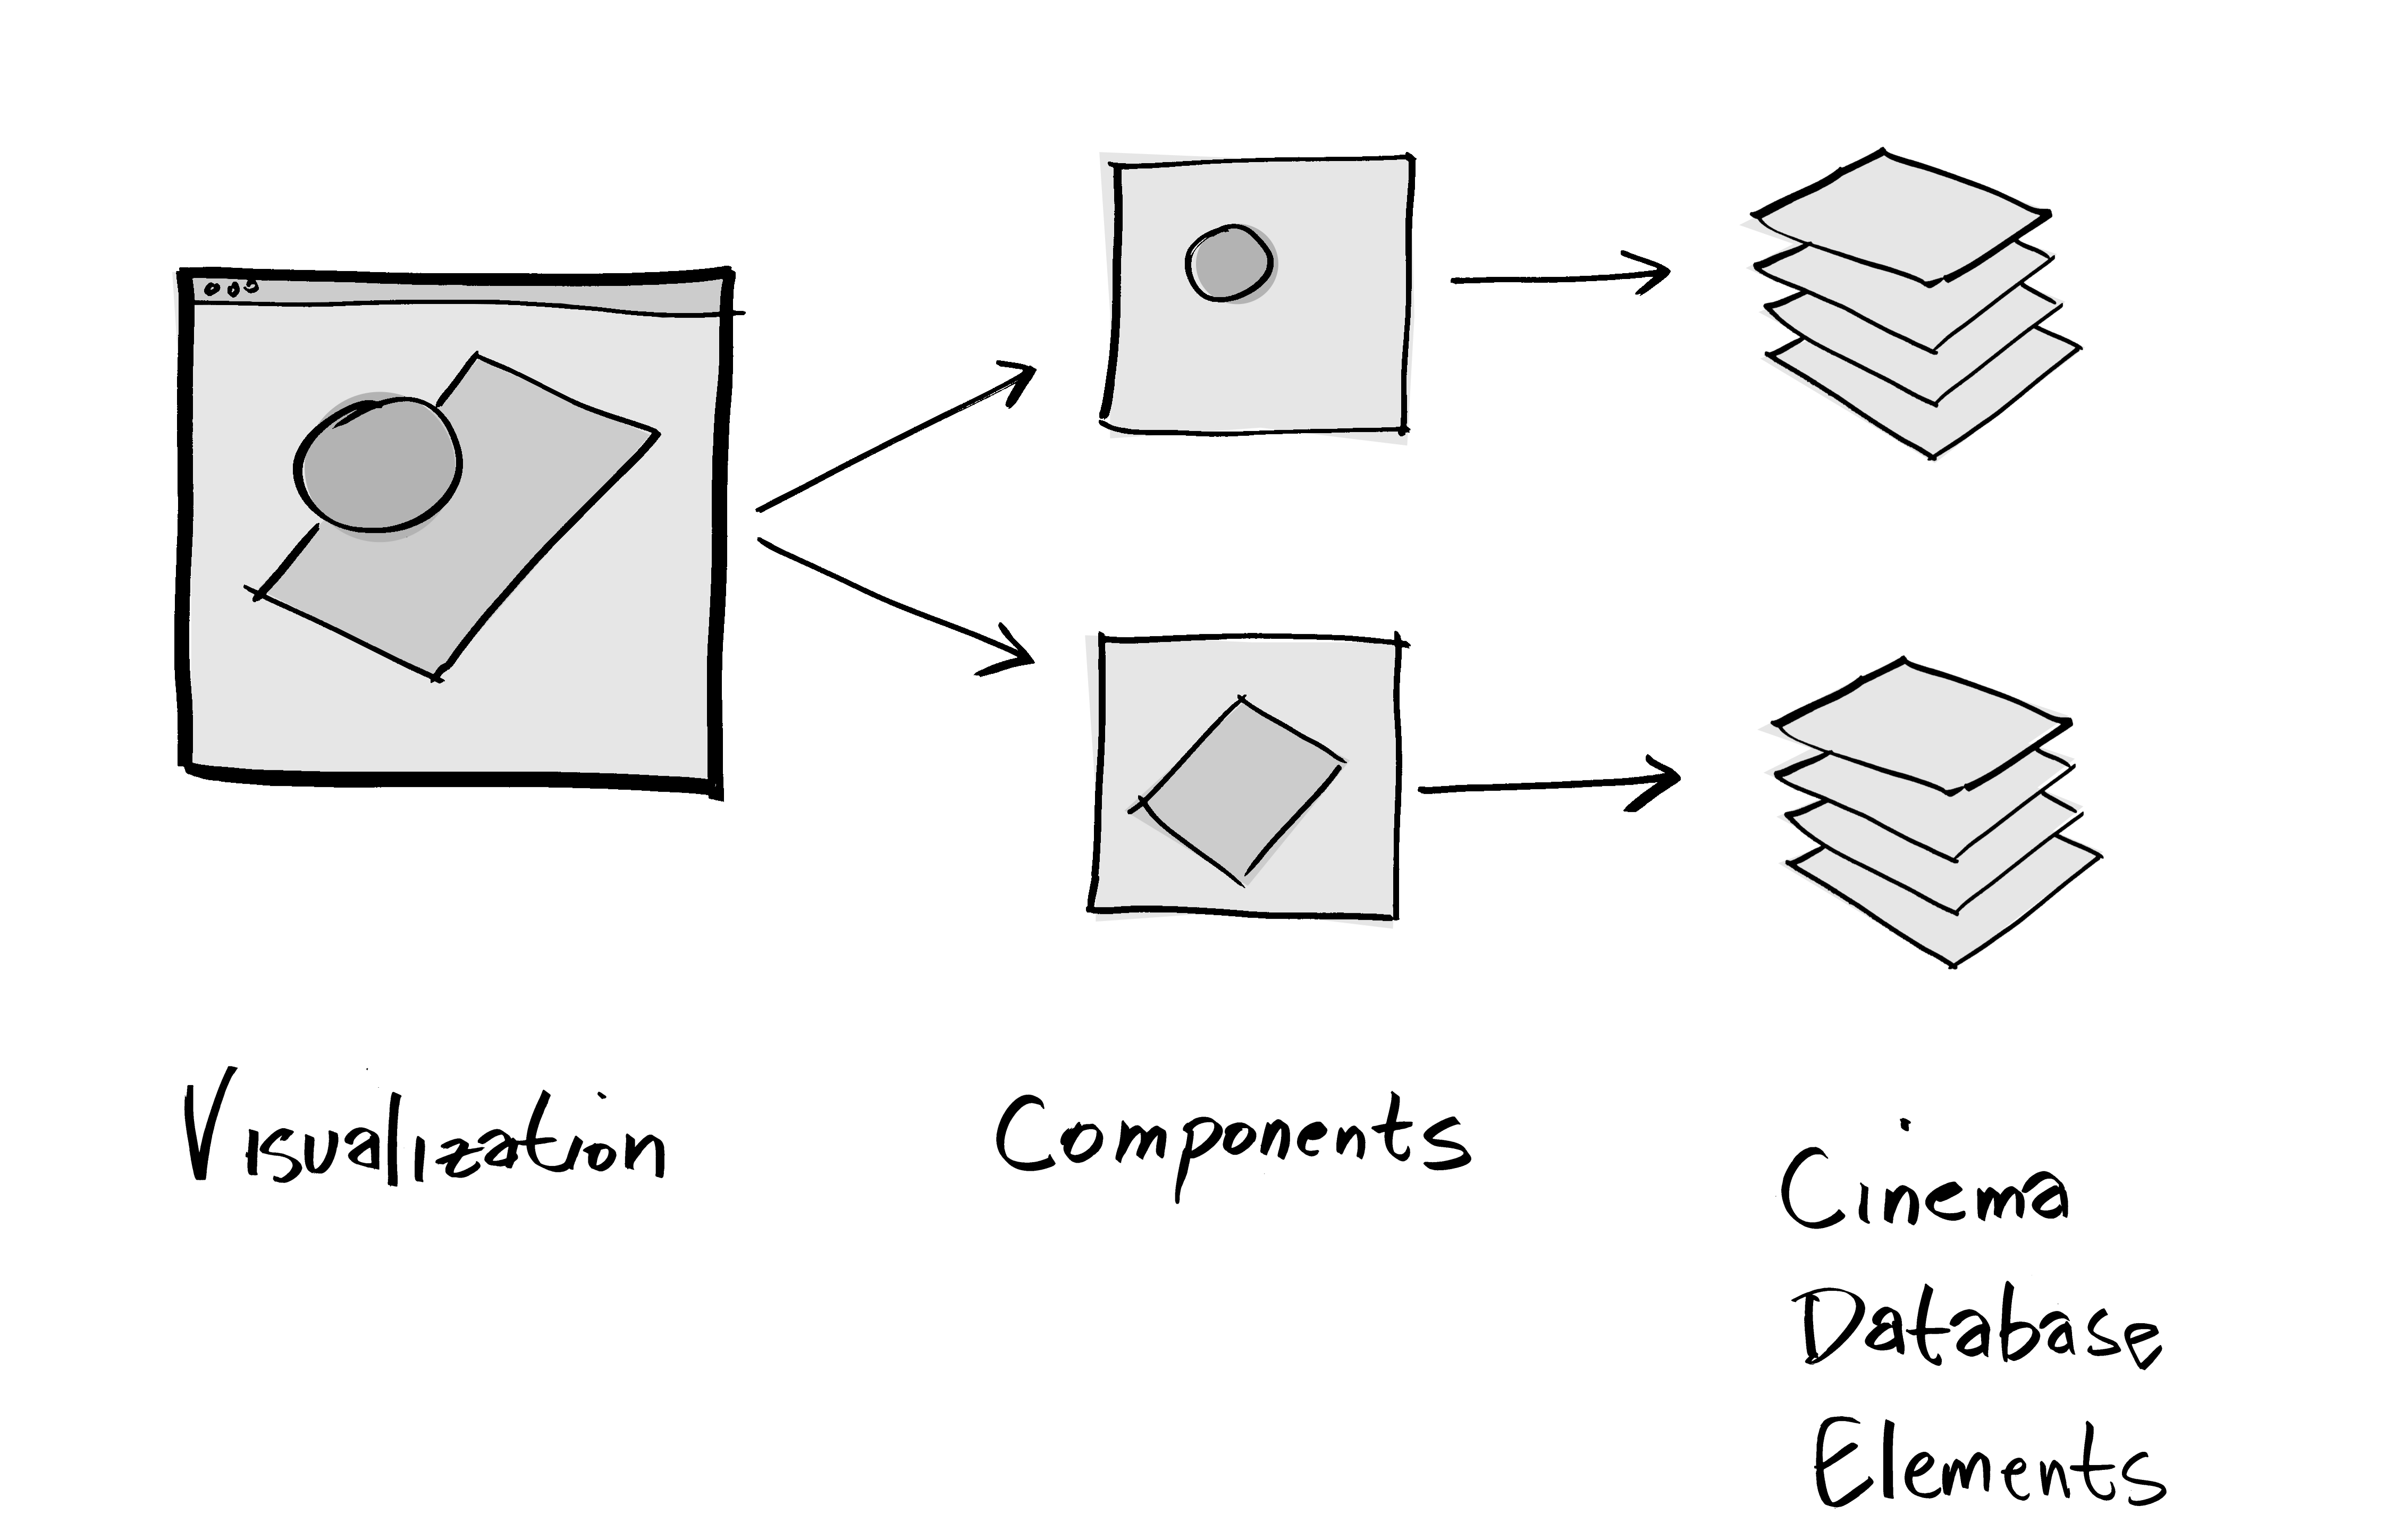
\includegraphics[width=0.8\textwidth]{img/image_pipeline_create_fill_labels}
\caption{
    Conceptual diagram of how to map a visualization to elements in a Cinema database. A user starts with a \textbf{visualization} that is to be saved as a Cinema database. The user first decides which \textbf{components} are desired, and what interactions are needed from the resulting database. This determines the \textbf{Cinema database elements} that must be created and saved according to this specification. Elements which are to be independently controlled, queried or analyzed are separately rendered as \textit{images}, and are written into the database as set of \textit{image channels}. The channels written into the database determine what operations are possible on the data when it is retrieved from the database for visualization, analysis or querying. See section~\ref{sec:image_channels} for more information on channels.
}
\label{fig:workflow_create}
\end{figure}


\begin{figure}[h!]
\centering
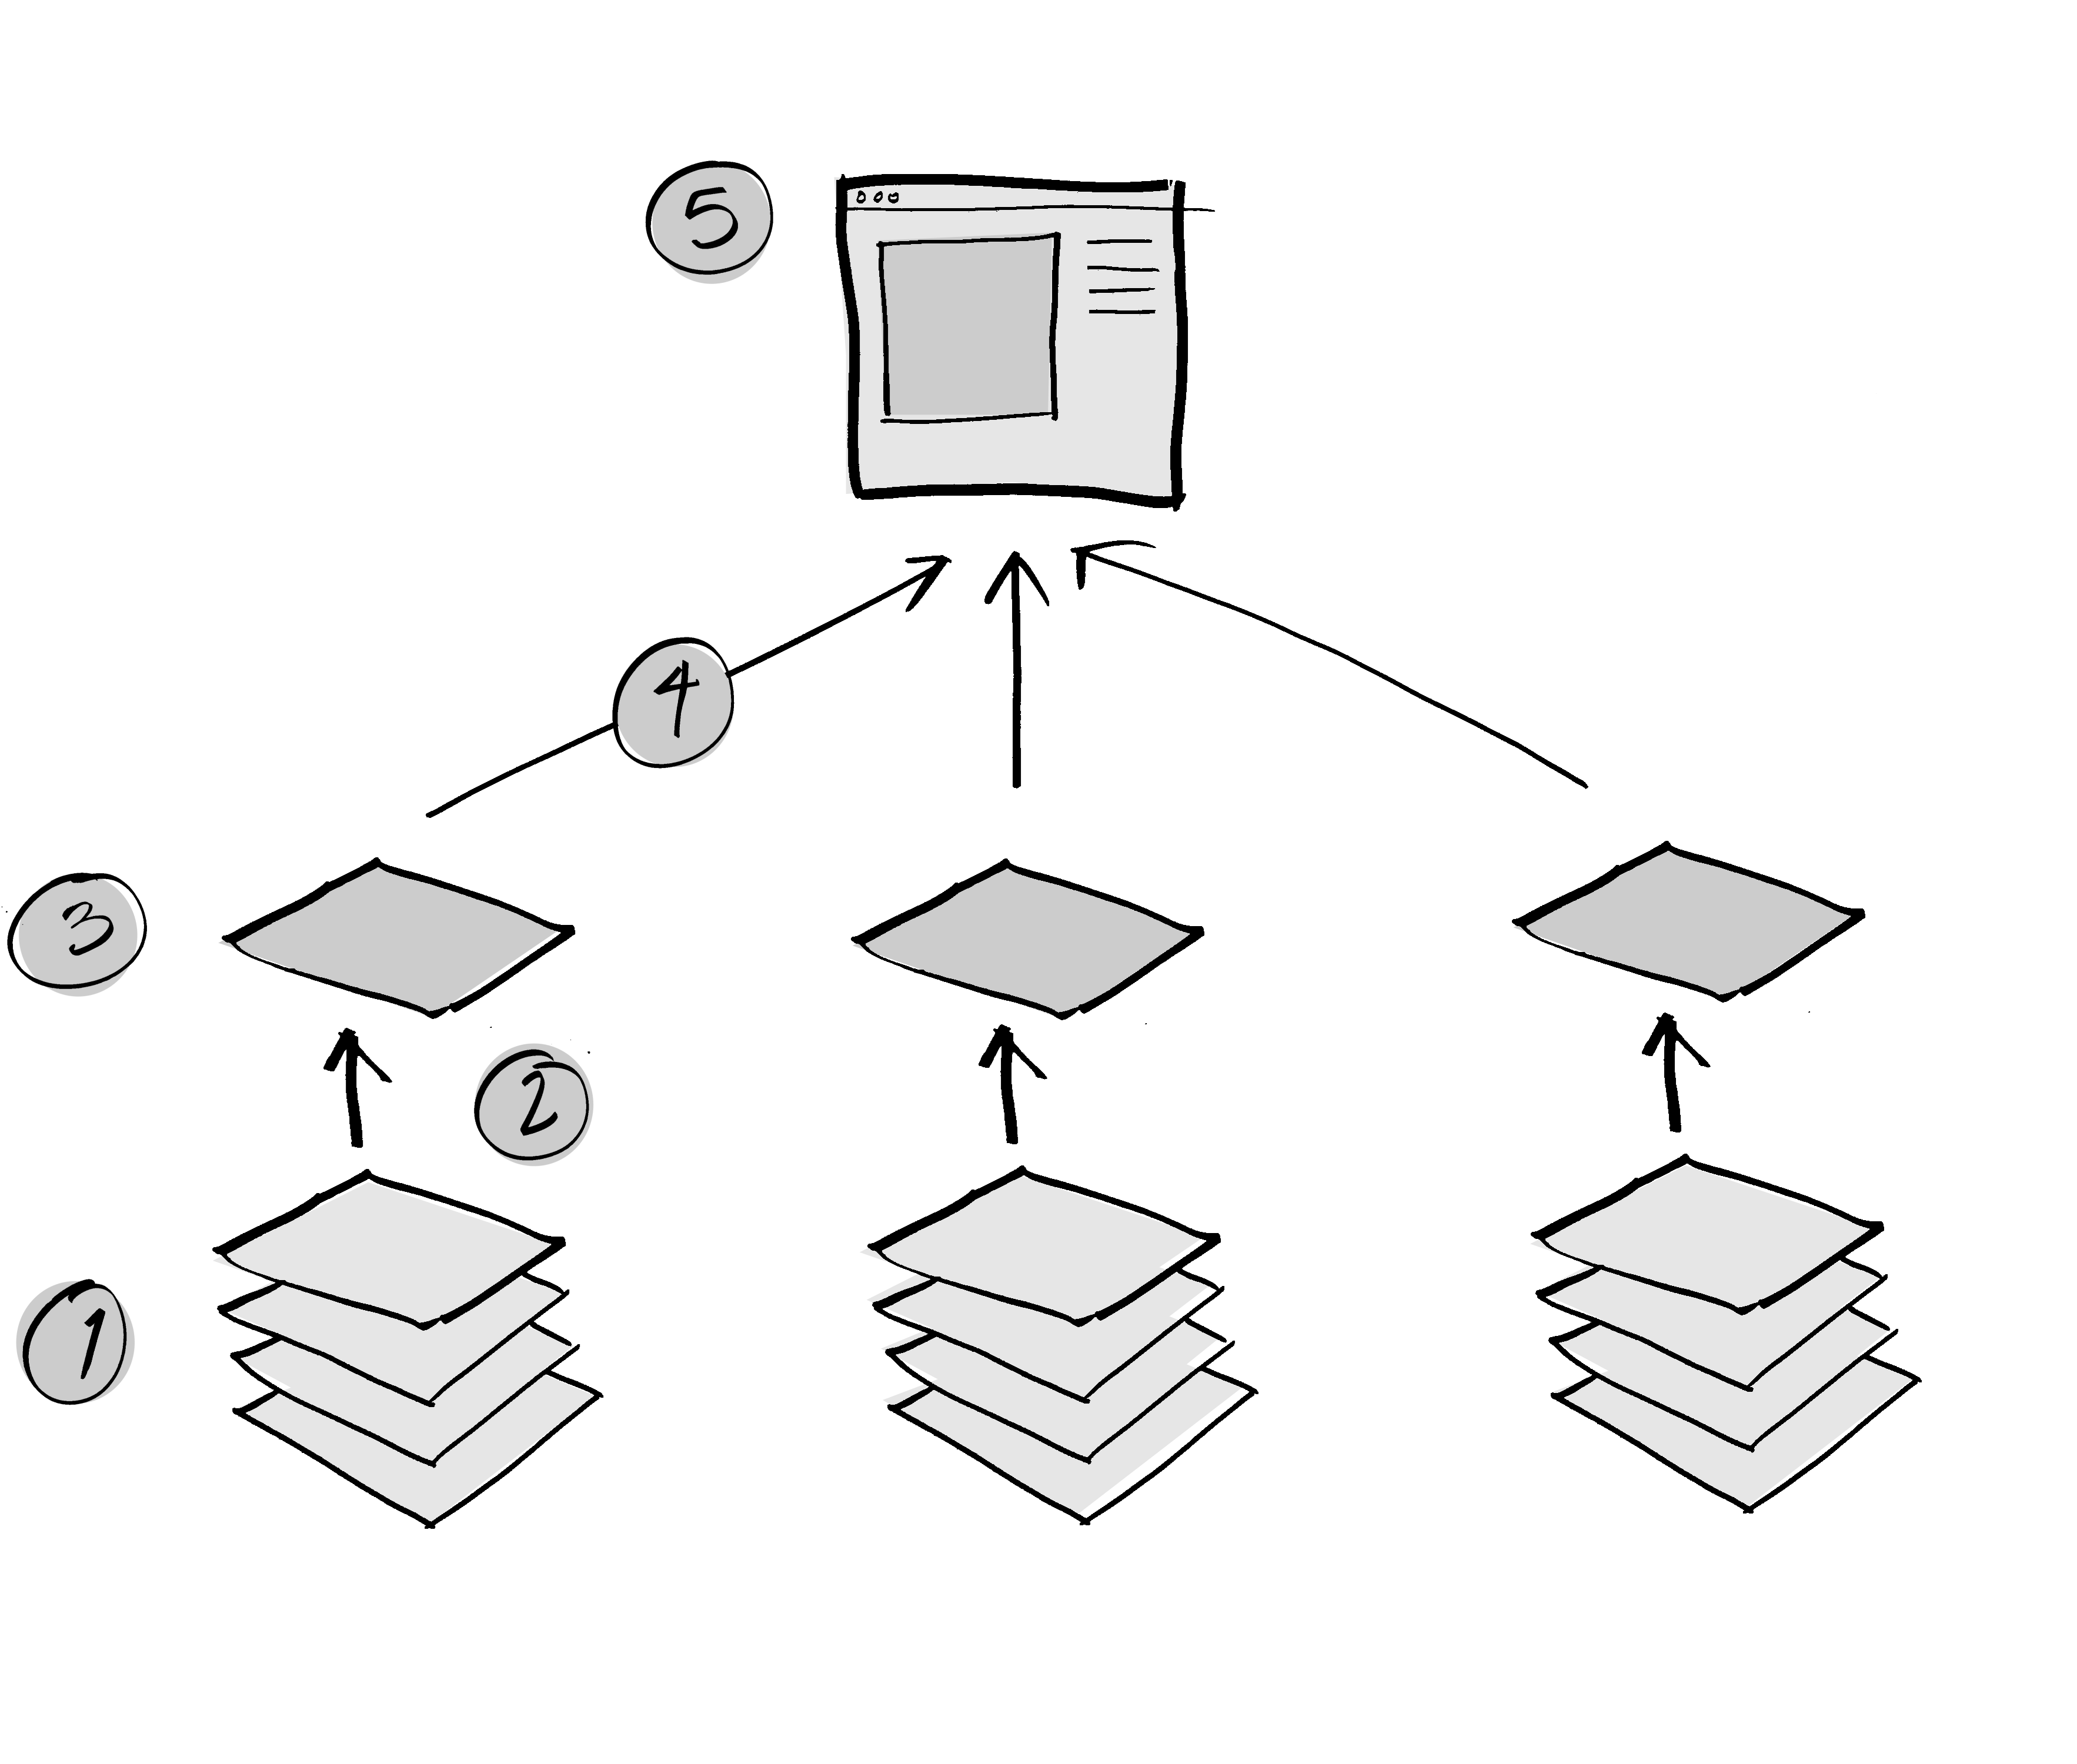
\includegraphics[width=0.8\textwidth]{img/image_pipeline_numbers_fill}
\caption{
    Diagrammatic workflow of components in a Cinema database. \textit{Image channels} (1) are gathered together in a \textit{fusion} operation (2) to create a single \textit{image} (3). The \textit{image channels} and the \textit{fusion} operation are described in section~\ref{sec:channels}. Any number of \textit{images} can then be combined together in a \textit{compositing operation} (4). The final product of that composite can be shown in a viewer application as a \textit{rendering} (5). The same data workflow can provide \textit{images} or \textit{renderings} to a query application, an analysis operator or other application.
}
\label{fig:workflow}
\end{figure}

\subsection{What is a Cinema Database?}
A Cinema database is a set of precomputed visualization components that can be queried and interactively viewed. The user can decide what types of components comprise the database, based on the type of interaction that is desired with the final database.  Figure~\ref{fig:workflow_create} shows a diagram of the way in which final renderings are broken into components, and then finally to image channels that this specification expects. For more detail on the types of interactions that you might create, see \cite{cinemaSC14}. Once a Cinema database is created, a user can create a viewer or analysis operator that somehow makes use of the data. A diagram of this is shown Figure~\ref{fig:workflow}. One application that can be created is an interactive viewer that allows a scientist to interactively view the data, as described in \cite{cinemaSC14}. This specification describes data which could be used by such a viewer, but could be ignored by other applications. This is a general design philosophy of Cinema - applications that read a Cinema database can ignore data, read subsets of channels, and otherwise determine which operations to perform. This promotes a wide range of possible interactions with the data.

\todo{DHR: examples of these}

This document describes release \CinemaSpecVersion of the Cinema \chaplin Database, in which image channels are stored instead of standalone fully pre-rendered images. The constituent images are inputs to a deferred rendering algorithm which allows the user to control which objects are in view and how each is colored. 

\subsubsection{Parameters in Cinema}
\label{sec:parameters}

A Cinema database holds a collection of results sampled by a set of visualization parameters. Visualization parameters can be created for any control that the user might have in a traditional visualization session. Examples include isosurfaces, slice planes and viewpoint. Cinema viewing applications give the user a control for each parameter setting and display the corresponding precomputed results, as if the user had made the same choices in a traditional visualization tool from the full resolution input data. As cinema holds only images, it is much more lightweight and display is always a constant time operation regardless of the parameter that is being changed.

Examples of typical parameters in a cinema database are:
\begin{itemize}
\item \textbf{Time}. Time varying data can be sampled at arbitrary points along the temporal domain.
\item \textbf{Camera positions}. In a static camera, the position and orientation is fixed. In a spherical camera, the position varies over a set of positions centered around a chosen focal point. More complicated camera tracks are possible.
\item \textbf{Visualization Operators}. Many visualization approaches use a data pipeline model that can apply operators such as clipping planes and isocontours. These can be rendered as individual elements that can be shown or hidden when viewing a cinema database.
\end{itemize}

\subsubsection{Cinema Image Channels}
\label{sec:channels}
In a Cinema workflow, the application producing a Cinema Database creates a set of image channels for each sample in the parameter space. Technically it does so by iterating over all assigned values for the color parameter of the currently displayed object and capturing each image. Likewise viewing applications let the user choose an object, take in the set of color results for that object and use them to draw that object on the screen. Each channel is written to disk as an image file, and these are fused together to create a 'normal' image. The fusion operation depends on which channels are present, and this is detailed in later sections. 

Figure~\ref{fig:workflow} shows a diagrammatic workflow for pulling data from a cinema database. An application or library pulls specific images from the database, based on some set of parameters. These images result from fusing several \textit{image channels} from the database. These are described in more detail in section~\ref{sec:image_channels}.

\subsubsection{Cinema Metadata}
In addition to the sampled data, a cinema database contains metadata that describes what the samples are, how they are stored and how they can be used. It must:
\begin{itemize}
\item identify the specific format (version number and content type) of the Cinema database,
\item identify specific storage formats for any artifacts in the database (for example, images),
\item enumerate the entire set of parameters that are explorable in the database and describe relationships between the parameters where they exist,
\item enable applications to map parameter value combinations to storage locations,
\item annotate parameters as necessary to indicate how they need to be handled
\end{itemize}
